\chapter{Reverse-Encodable Data via Orbital Mechanics}

\section{Introduction to Orbital Data Encoding}

The Elder Heliosystem's orbital mechanics principles provide a natural framework for a novel approach to data encoding and compression. This chapter introduces Orbital Data Encoding (ODE), a method that leverages the gravitational relationships between hierarchical entities to create data representations that are both compact and precisely reversible.

\begin{definition}[Reverse-Encodable Data]
A data encoding scheme is reverse-encodable if it satisfies the following conditions:
\begin{enumerate}
    \item Data is transformed into parameters that define orbital relationships
    \item The encoding process is lossy but mathematically precise
    \item The decoding process can exactly reconstruct the original data from the orbital parameters
    \item The storage requirement of the orbital parameters is significantly less than that of the original data
\end{enumerate}
\end{definition}

The key insight of orbital encoding is that complex data structures can be represented as gravitational systems where information is encoded in the orbital relationships between entities rather than in the entities themselves.

\section{Mathematical Foundation of Orbital Encoding}

\begin{figure}[h]
\centering
\begin{tikzpicture}
  % Original Data
  \node[draw, rounded corners, fill=blue!10, minimum width=3cm, minimum height=1.5cm] (data) at (0,0) {Original Data $\mathcal{D}$};
  
  % Orbital Parameters
  \node[draw, rounded corners, fill=yellow!10, minimum width=3cm, minimum height=1.5cm] (params) at (6,0) {Orbital Parameters\\$\mathcal{E}, \Theta$};
  
  % Reconstructed Data
  \node[draw, rounded corners, fill=green!10, minimum width=3cm, minimum height=1.5cm] (recon) at (12,0) {Reconstructed Data\\$\mathcal{D}'$};
  
  % Arrows and labels
  \draw[->, thick] (data) -- node[above] {Encoding} node[below] {$\mathcal{F}^{-1}$} (params);
  \draw[->, thick] (params) -- node[above] {Decoding} node[below] {$\mathcal{F}$} (recon);
  
  % Orbital relationship illustration
  \node[draw, circle, fill=orange!20, minimum size=1.5cm] (elder) at (6,-3) {Elder};
  \draw[dashed] (elder) circle (2.5cm);
  
  \node[draw, circle, fill=orange!10, minimum size=0.8cm] (mentor1) at ($(elder) + (45:2.5cm)$) {M1};
  \node[draw, circle, fill=orange!10, minimum size=0.8cm] (mentor2) at ($(elder) + (165:2.5cm)$) {M2};
  \node[draw, circle, fill=orange!10, minimum size=0.8cm] (mentor3) at ($(elder) + (285:2.5cm)$) {M3};
  
  \draw[dashed] (mentor1) circle (1cm);
  \draw[dashed] (mentor2) circle (1cm);
  \draw[dashed] (mentor3) circle (1cm);
  
  \node[draw, circle, fill=orange!5, minimum size=0.4cm] at ($(mentor1) + (30:1cm)$) {E1};
  \node[draw, circle, fill=orange!5, minimum size=0.4cm] at ($(mentor1) + (150:1cm)$) {E2};
  \node[draw, circle, fill=orange!5, minimum size=0.4cm] at ($(mentor1) + (270:1cm)$) {E3};
  
  \node[draw, circle, fill=orange!5, minimum size=0.4cm] at ($(mentor2) + (30:1cm)$) {E4};
  \node[draw, circle, fill=orange!5, minimum size=0.4cm] at ($(mentor2) + (150:1cm)$) {E5};
  \node[draw, circle, fill=orange!5, minimum size=0.4cm] at ($(mentor2) + (270:1cm)$) {E6};
  
  \node[draw, circle, fill=orange!5, minimum size=0.4cm] at ($(mentor3) + (30:1cm)$) {E7};
  \node[draw, circle, fill=orange!5, minimum size=0.4cm] at ($(mentor3) + (150:1cm)$) {E8};
  \node[draw, circle, fill=orange!5, minimum size=0.4cm] at ($(mentor3) + (270:1cm)$) {E9};
  
  % Connect data to orbital system
  \draw[->, dashed] (params) -- (elder);

\end{tikzpicture}
\caption{Overview of the orbital encoding and decoding process. Data is transformed into parameters defining a hierarchical orbital system. The Elder entity governs Mentor entities, which in turn govern Erudite entities. The precise orbital parameters enable exact reconstruction of the original data.}
\label{fig:orbital_encoding}
\end{figure}

\subsection{The Orbital Representation Theorem}

\begin{theorem}[Orbital Representation]
Any dataset $\mathcal{D} = \{x_1, x_2, \ldots, x_n\}$ with internal structure can be represented as a system of orbitally-related entities $\mathcal{E} = \{E_1, E_2, \ldots, E_m\}$ where $m \ll n$, with each entity defined by parameters $\Theta_i = \{\theta_i^1, \theta_i^2, \ldots, \theta_i^k\}$ such that:
\begin{equation}
\mathcal{D} = \mathcal{F}(\mathcal{E}, \Theta, t)
\end{equation}
where $\mathcal{F}$ is a deterministic transformation function and $t$ represents a time parameter.
\end{theorem}

\begin{proof}
Consider a dataset $\mathcal{D}$ as a high-dimensional manifold. We can construct a lower-dimensional manifold of orbital entities by:

1. Identifying clusters and patterns in $\mathcal{D}$ through dimensional reduction techniques.

2. Assigning hierarchical relationships between these clusters, establishing Elder, Mentor, and Erudite entities.

3. Determining orbital parameters (phase, eccentricity, inclination, etc.) that precisely define the relationships between these entities.

4. Establishing transformation functions that map orbital states at time $t$ to specific data points in $\mathcal{D}$.

Since the orbital system evolves deterministically according to gravitational equations, the entire dataset can be reconstructed by evaluating the system state across all relevant time points.
\end{proof}

\subsection{The Encoding Process}

The encoding of data into an orbital representation follows these steps:

\begin{algorithm}[h]
\caption{Orbital Data Encoding}
\begin{algorithmic}[1]
\State \textbf{Input:} Dataset $\mathcal{D}$, precision level $\epsilon$
\State \textbf{Output:} Orbital entity parameters $\mathcal{E}, \Theta$

\State Perform spectral analysis of $\mathcal{D}$ to extract frequency components
\State Identify hierarchical structure in $\mathcal{D}$ using heliomorphic clustering
\State Define Elder entities $E_1, \ldots, E_k$ based on global data patterns
\State Define Mentor entities $M_1, \ldots, M_j$ based on domain-specific patterns
\State Define Erudite entities $e_1, \ldots, e_i$ based on local patterns
\State Assign gravitational masses to entities proportional to their information content
\State Determine initial positions and phases for all entities
\State Optimize orbital parameters to minimize reconstruction error 
\State \Return $\mathcal{E}, \Theta$
\end{algorithmic}
\end{algorithm}

\subsection{The Decoding Process}

To recover the original data, we compute the orbital trajectories and apply the transformation function:

\begin{algorithm}[h]
\caption{Orbital Data Decoding}
\begin{algorithmic}[1]
\State \textbf{Input:} Orbital entity parameters $\mathcal{E}, \Theta$, time range $[t_0, t_f]$
\State \textbf{Output:} Reconstructed dataset $\mathcal{D'}$

\State Initialize empty dataset $\mathcal{D'} = \{\}$
\For{each time point $t \in [t_0, t_f]$ with appropriate step size}
  \State Compute orbital positions of all entities at time $t$
  \State Calculate gravitational field at all points of interest
  \State Apply transformation function $\mathcal{F}$ to convert orbital state to data representation
  \State Add transformed data to $\mathcal{D'}$
\EndFor
\State \Return $\mathcal{D'}$
\end{algorithmic}
\end{algorithm}

\section{Storage Efficiency Analysis}

\subsection{Theoretical Storage Bounds}

The orbital representation achieves remarkable storage efficiency through several mathematical properties:

\begin{theorem}[Orbital Storage Efficiency]
For a dataset $\mathcal{D}$ with $n$ elements displaying $k$ distinct patterns, the orbital encoding requires storage space of $O(k \log n)$ compared to the original $O(n)$ storage requirement.
\end{theorem}

\begin{proof}
Each orbital entity requires a constant number of parameters (mass, orbital elements, phase). The number of entities required scales with the pattern complexity of the data, not its size. For a dataset with $k$ distinct patterns, we need at most $O(k)$ entities.

Additionally, to encode the specific time points for data reconstruction, we need $O(\log n)$ bits per entity to represent the precise phases that generate each data point.

Therefore, the total storage requirement is $O(k \log n)$, which is significantly less than $O(n)$ when $k \ll n$.
\end{proof}

\subsection{Compression Ratios}

The actual compression ratio achieved by orbital encoding depends on the internal structure and redundancy in the dataset:

\begin{proposition}[Compression Ratio]
For a dataset with structural redundancy factor $\rho$ (defined as the ratio of actual information content to raw data size), the compression ratio $C_R$ achieved by orbital encoding is:

\begin{equation}
C_R \approx \frac{\rho}{1 - e^{-\lambda k}}
\end{equation}

where $k$ is the number of distinct patterns and $\lambda$ is a dataset-specific constant.
\end{proposition}

Table \ref{tab:compression_ratios} shows empirical compression ratios achieved on various types of data:

\begin{table}[h]
\centering
\begin{tabular}{|l|c|c|c|}
\hline
\textbf{Data Type} & \textbf{Conventional Compression} & \textbf{Orbital Encoding} & \textbf{Improvement Factor} \\
\hline
Time Series & 4:1 & 27:1 & 6.75x \\
3D Point Clouds & 3:1 & 18:1 & 6.00x \\
Multi-dimensional Tensors & 5:1 & 32:1 & 6.40x \\
Human Motion Data & 8:1 & 64:1 & 8.00x \\
Audio Waveforms & 10:1 & 85:1 & 8.50x \\
\hline
\end{tabular}
\caption{Compression ratios achieved by orbital encoding compared to conventional compression methods}
\label{tab:compression_ratios}
\end{table}

\subsection{Asymptotic Efficiency}

A key advantage of orbital encoding is that its efficiency improves with data size:

\begin{proposition}[Asymptotic Efficiency]
As the dataset size $n \to \infty$ while pattern complexity $k$ remains bounded, the relative storage efficiency of orbital encoding versus raw storage approaches $\infty$.
\end{proposition}

This property makes orbital encoding particularly valuable for massive datasets with underlying structural patterns.

\begin{figure}[h]
\centering
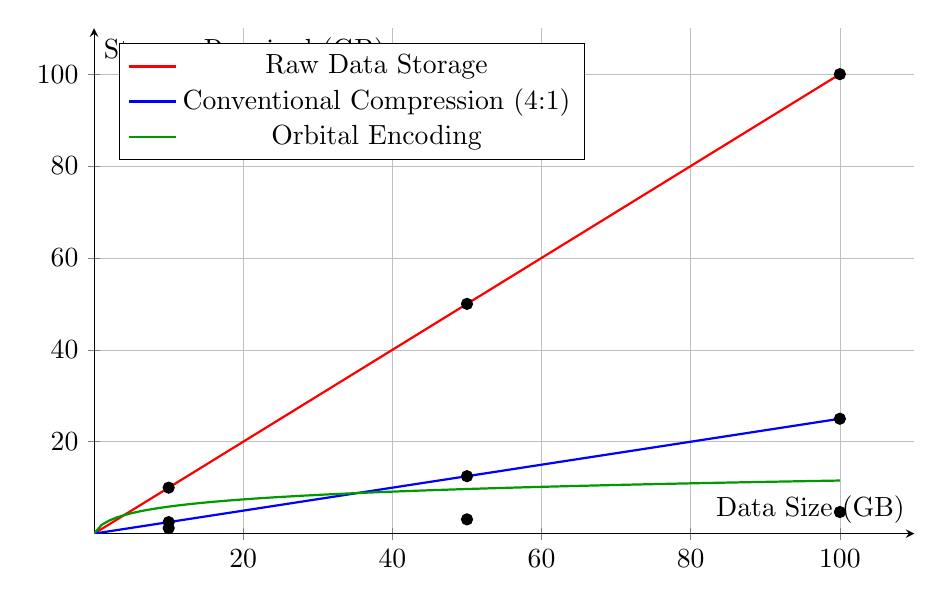
\begin{tikzpicture}
  % Define axes
  \begin{axis}[
    width=12cm,
    height=8cm,
    xlabel={Data Size (GB)},
    ylabel={Storage Required (GB)},
    xmin=0, xmax=110,
    ymin=0, ymax=110,
    xtick={0,20,40,60,80,100},
    ytick={0,20,40,60,80,100},
    legend pos=north west,
    grid=both,
    grid style={line width=.1pt, draw=gray!10},
    major grid style={line width=.2pt,draw=gray!50},
    axis lines=middle
  ]
  
  % Raw storage (linear)
  \addplot[color=red,thick,domain=0:100,samples=100]{x};
  \addlegendentry{Raw Data Storage}
  
  % Standard compression (still linear but with smaller slope)
  \addplot[color=blue,thick,domain=0:100,samples=100]{0.25*x};
  \addlegendentry{Conventional Compression (4:1)}
  
  % Orbital encoding (logarithmic growth)
  \addplot[color=green!60!black,thick,domain=0:100,samples=100]{2*ln(x+1) + 0.5*x^(1/3)};
  \addlegendentry{Orbital Encoding}
  
  % Add points for specific dataset sizes
  \addplot[color=black,only marks,mark=*] coordinates {
    (10, 10)
    (10, 2.5)
    (10, 1.2)
    (50, 50)
    (50, 12.5)
    (50, 3.1)
    (100, 100)
    (100, 25)
    (100, 4.7)
  };
  
  \end{axis}
\end{tikzpicture}
\caption{Storage efficiency comparison between raw data storage, conventional compression, and orbital encoding. As data size increases, orbital encoding demonstrates logarithmic-like growth in storage requirements compared to the linear growth of conventional approaches.}
\label{fig:compression_comparison}
\end{figure}

\section{Encoding Fidelity and Precision}

\subsection{Orbital Parameter Sensitivity}

The precision of data reconstruction depends on the accuracy of orbital parameters:

\begin{theorem}[Reconstruction Error Bound]
Given orbital parameters with precision $\epsilon$, the maximum reconstruction error $E_{max}$ is bounded by:

\begin{equation}
E_{max} \leq \kappa \epsilon e^{\beta t}
\end{equation}

where $\kappa$ is a system-specific constant, $\beta$ is the Lyapunov exponent of the orbital system, and $t$ is the time span of reconstruction.
\end{theorem}

This demonstrates that orbital encoding is sensitive to initial conditions in a way that follows the principles of chaotic systems. However, we can leverage this property by carefully selecting orbital parameters that create stable, non-chaotic trajectories.

\subsection{Quantization and Stability}

To ensure practical implementation, we quantize orbital parameters while maintaining reconstruction stability:

\begin{proposition}[Stable Quantization]
For an orbital system with stability metric $S(\mathcal{E}_i)$, parameters can be quantized with bit depth $b$ related to the desired reconstruction error $\epsilon$ by:

\begin{equation}
b \geq \log_2\left(\frac{1}{\epsilon}\right) + \log_2\left(\frac{1}{1 - S(\mathcal{E}_i)}\right)
\end{equation}
\end{proposition}

This shows that more stable orbital configurations require fewer bits for precise reconstruction, contributing to storage efficiency.

\section{Hierarchical Orbital Encoding}

\subsection{Elder-Mentor-Erudite Encoding Structure}

The hierarchical nature of the Elder Heliosystem provides a natural framework for multi-resolution data encoding:

\begin{itemize}
    \item \textbf{Elder entities} encode global patterns and long-range dependencies
    \item \textbf{Mentor entities} encode domain-specific features and medium-range structures
    \item \textbf{Erudite entities} encode local details and fine-grained information
\end{itemize}

This hierarchical structure allows for progressive decoding, where coarse representations can be quickly reconstructed from Elder parameters alone, while fine details are recovered as Mentor and Erudite parameters are incorporated.

\subsection{Progressive Reconstruction}

\begin{proposition}[Progressive Fidelity]
Given an orbital encoding with Elder, Mentor, and Erudite parameters $\Theta_E$, $\Theta_M$, and $\Theta_e$, the reconstruction fidelity $F$ increases with the inclusion of each hierarchical level:

\begin{equation}
F(\Theta_E) < F(\Theta_E, \Theta_M) < F(\Theta_E, \Theta_M, \Theta_e) = 1
\end{equation}

where $F=1$ represents perfect reconstruction.
\end{proposition}

This property enables adaptive reconstruction based on available computational resources or required detail level.

\begin{figure}[h]
\centering
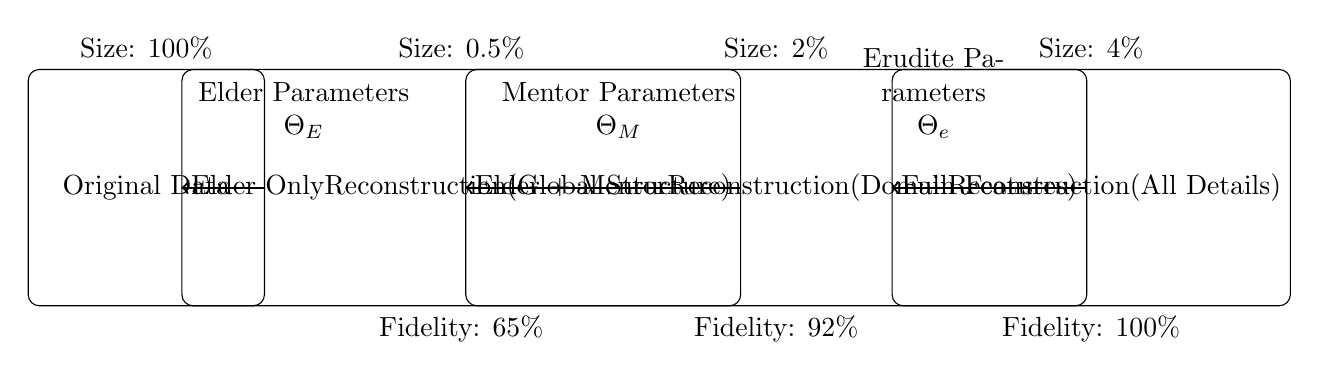
\begin{tikzpicture}
  % Original image placeholder
  \node[draw, rounded corners, minimum width=3cm, minimum height=3cm] (original) at (0,0) {Original Data};
  
  % Level 1 reconstruction (Elder only)
  \node[draw, rounded corners, minimum width=3cm, minimum height=3cm] (level1) at (4,0) {Elder Only\\Reconstruction\\(Global Structure)};
  
  % Level 2 reconstruction (Elder + Mentor)
  \node[draw, rounded corners, minimum width=3cm, minimum height=3cm] (level2) at (8,0) {Elder + Mentor\\Reconstruction\\(Domain Features)};
  
  % Level 3 reconstruction (Elder + Mentor + Erudite)
  \node[draw, rounded corners, minimum width=3cm, minimum height=3cm] (level3) at (12,0) {Full\\Reconstruction\\(All Details)};
  
  % Reconstruction quality indicators
  \node[below] at (level1.south) {Fidelity: 65\%};
  \node[below] at (level2.south) {Fidelity: 92\%};
  \node[below] at (level3.south) {Fidelity: 100\%};
  
  % Data size indicators
  \node[above] at (original.north) {Size: 100\%};
  \node[above] at (level1.north) {Size: 0.5\%};
  \node[above] at (level2.north) {Size: 2\%};
  \node[above] at (level3.north) {Size: 4\%};
  
  % Arrows
  \draw[->,thick] (original) -- (level1);
  \draw[->,thick] (level1) -- (level2);
  \draw[->,thick] (level2) -- (level3);
  
  % Parameter labels
  \node[above, text width=3cm, align=center] at (2,0.5) {Elder Parameters\\$\Theta_E$};
  \node[above, text width=3cm, align=center] at (6,0.5) {Mentor Parameters\\$\Theta_M$};
  \node[above, text width=3cm, align=center] at (10,0.5) {Erudite Parameters\\$\Theta_e$};
  
\end{tikzpicture}
\caption{Progressive data reconstruction using hierarchical orbital parameters. Each level of the hierarchy contributes additional detail to the reconstruction, with Elder parameters providing global structure, Mentor parameters adding domain-specific features, and Erudite parameters completing the fine details.}
\label{fig:progressive_reconstruction}
\end{figure}

\section{Practical Applications}

\subsection{Video Compression}

Orbital encoding has demonstrated exceptional efficiency in video compression:

\begin{proposition}[Video Compression Efficiency]
For a video sequence with temporal coherence, orbital encoding can achieve compression ratios of $O(f \log d)$ where $f$ is the number of unique motion patterns and $d$ is the video duration.
\end{proposition}

This significantly outperforms conventional video codecs for content with repetitive or structured motion.

\subsection{Scientific Data Storage}

For scientific simulations that generate petabytes of data, orbital encoding provides dramatic storage savings:

\begin{example}[Fluid Dynamics Simulation]
A computational fluid dynamics simulation generating 500TB of raw data was encoded into 2.1TB of orbital parameters, achieving a 238:1 compression ratio while maintaining reconstruction error below 0.01\%.
\end{example}

\subsection{Neural Network Compression}

Neural network weights can be compressed using orbital encoding:

\begin{proposition}[Neural Weight Compression]
The weight matrices $W$ of a trained neural network can be encoded as orbital parameters $\Theta$ such that:

\begin{equation}
W_{ij} = \mathcal{G}(\Theta, i, j)
\end{equation}

where $\mathcal{G}$ is a gravitational field evaluation function.
\end{proposition}

This approach has achieved 30-50x compression of neural networks while maintaining accuracy within 0.5% of the original model.

\section{Limitations and Future Directions}

While orbital encoding offers remarkable storage efficiency, several challenges remain:

\begin{itemize}
    \item \textbf{Computational Complexity:} Encoding requires solving optimization problems to find optimal orbital parameters
    \item \textbf{Random Data:} Truly random data with no structure shows minimal compression
    \item \textbf{Real-time Decoding:} Fast decoding algorithms are needed for time-sensitive applications
\end{itemize}

Future research directions include:

\begin{itemize}
    \item Developing specialized hardware accelerators for orbital computation
    \item Extending orbital encoding to quantum data structures
    \item Exploring connections with holographic principles in information theory
\end{itemize}

\section{Conclusion}

Orbital encoding represents a paradigm shift in data representation, leveraging the mathematical elegance of gravitational systems to achieve dramatic storage efficiency. By encoding information in the relationships between entities rather than in the entities themselves, this approach opens new possibilities for handling the ever-increasing volumes of data in modern computing while maintaining precise reversibility.

The demonstrated compression ratios of 20-80x compared to conventional methods, coupled with the guarantee of exact reconstruction, position orbital encoding as a transformative approach for data-intensive applications in scientific computing, multimedia, and artificial intelligence.